\chapter{Lecture \thechapter{} of 08/04/2026}

Let $C \seq \Rnp$, $x \notin C$. \underline{Idea}: if $C$ does not contain vertical lines, we can striclty separate $C$ from $x$ with a ''non-vertical'' hyperplane. 

For $(u,w) \in \Rnp$, $u \in \Rn$, $w \in \R$. An hyperplane $H$ is in the form 

\[ H = \set{(u,w) : (u,w)^\top \cdot (\mu,\beta) = b} \]

for $\mu \in \Rn$, $\beta \in \R$. We say that $H$ is nonvertical if $\beta \neq 0$.

\begin{figure}[ht!]
    \centering
    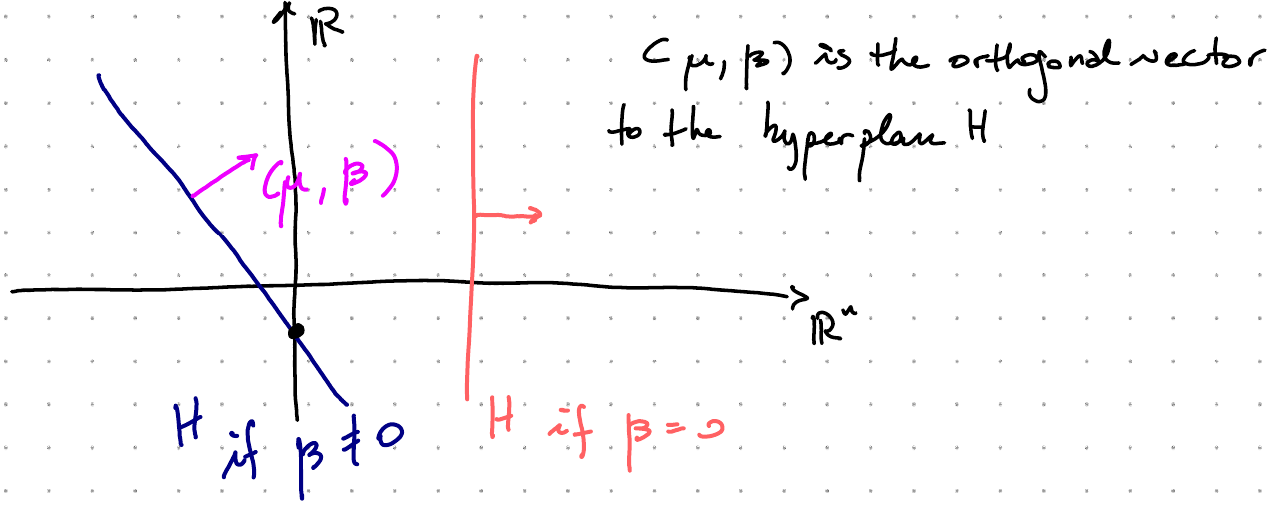
\includegraphics[width=0.8\textwidth]{img/hyperplane_nv.png}
\end{figure}

If $(\bar{u},\bar{w}) \in H$, then $H = (\bar{u},\bar{w}) + (u,w)$ such that $(u,w) \perp (\mu,\beta)$ (i.e. $(u,w)^\top \cdot (\mu,\beta) = 0$).

Which is the height at which $H$ intersects the $(n+1)$-axis? When the point $(0,\xi) \in H$? If $(0,\xi) = (\bar{u},\bar{w}) + (u,w)$ for $(u,w)\perp(\mu,\beta)$. Multiply by $(\mu,\beta)$, i.e. take the projection, so 

\[ \xi \beta = \bar{u}^\top \cdot \mu + \beta \bar{w} + 0 \implies \xi = \frac{\bar{u}^\top\cdot\mu}{\beta} + \bar{w}. \]

\begin{proposition}[Non-vertical hyperplane theorem, book 1.5.8]

    Let $C \seq \Rnp$ nonempty convex set, assume $C$ does not contain any vertical line. Then

    \begin{enumerate}
        \item $C$ is contained in the closed halfspace corresponding to a non-vertical hyperplane, i.e there exists $\mu \in \Rn$, $0 \neq \beta \in \R$ and $\gamma \in \R$ such that 
            \[ \mu^\top u + \beta w \ge \gamma \quad \forall (u,w) \in C; \]
        \item if $(\bar{u},\bar{w}) \notin \cl{C}$, there exists a non-vertical hyperplane that striclty separates $(\bar{u},\bar{w})$ and $C$.
    \end{enumerate}
    
\end{proposition}

\begin{proof}
    Not required.
\end{proof}

\section{Convex conjugate functions}

We would like to describe a funciton $f$ as the supremum of a family of affine functions.

\begin{definition}
    
    Let $f : \Rn \to \Rb$. We define the \emph{conjugate} of $f$ (or convex conjugate) as the function 

    \[ f^*(y) = \sup_{x \in \Rn} y^\top x - f(x). \]

\end{definition}

\begin{figure}[ht!]
    \centering
    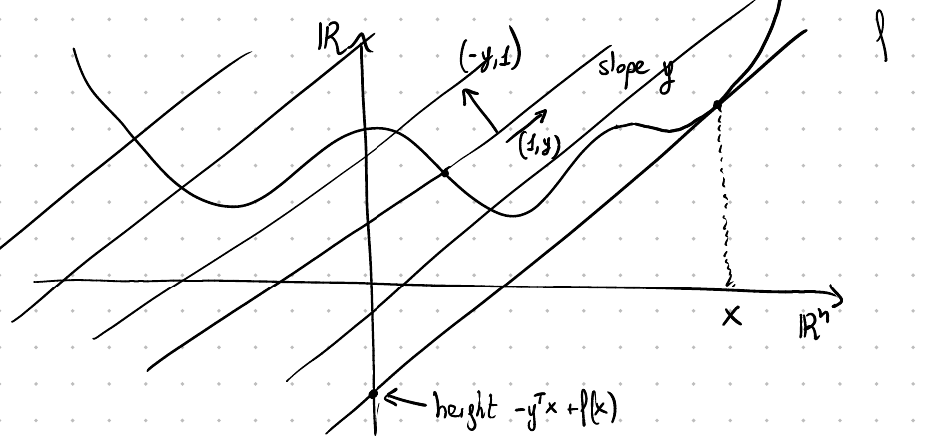
\includegraphics[width=0.8\textwidth]{img/conjugate.png}
\end{figure}

So what? Assume $f$ given. We want to describe $f$ as $\sup$\{affine function below $f$\} = $\sup$\{lines of any slope $y \in \Rn$, lines below $f$\}.

Fix a slope $y \in\Rn$ and fix any $(x,f(x))$ in the graph of $f$. Then the line passing through $(x,f(x))$ and of slope $y$ is 

\[ \set{(x,f(x)) + (u,w) : (u,w) \perp (-y,1)} \]

where the ''line'' $(x,f(x)) + (u,w)$ intersects $(0,\xi)$ at height $-y^\top x + f(x)$. 

To keep $f$ above the selected line of slope $y$, we need to use the one such that the quantity $-y^\top x + f(x)$ is infimized, so $\inf_{x \in \Rn} - y^\top x + f(x)$ is the intercept of the ''highest'' line with slope $y$ that passes from a point in the graph of $f$ and contains the graph of $f$ in one of its closed halfspaces. Now we observe that 

\[ \inf_{x \in \Rn} -y^\top x + f(x) = \sup_{x \in \Rn} y^\top x - f(x) = -f^*(y). \]

\begin{definition}[Biconjugate function]

    The biconjugate funciton is defined as 

    \[ f^{**}(x) = \sup_{y \in \Rn} x^\top y - f^*(y). \]
    
\end{definition}

\begin{example}
    
    Let $f(x) = x^2$. We want to compute its conjugate $f^*$. 

    From the definition, $f^*(y) = \sup_{x \in \Rn} \set{yx - f(x)}$. One strategy can be find the critical points of the function $g(x) = yx - x^2 \implies g^\prime(x)=y - 2x \implies x = y/2$ is a critical point (in particular a maximum). Hence 
    
    \[ f^*(y) = y \frac{y}{2} - (\frac{y}{2})^2 = \frac{y^2}{4}. \]

\end{example}

\begin{example}
    
    Let $f(x) = e^x$. Again, we can compute $g^\prime(x)$ and find a critical point:

    \[ g(x) = yx - e^x \implies g^\prime(x) = y-e^x \implies y = e^x \text{ critical point}. \]

    Now, if $y > 0$ we are fine, since $x = \log(y)$. Otherwise? If $y < 0$ we would have $yx - e^x = \text{ negative }\cdot x - e^x$ which explodes to $+\infty$ as $x \to -\infty$. If instead $y=0$, $\sup_x -e^x = 0$. Finally, 

    \[ 
        f^*(y) = 
        \begin{cases}
            y\log(y) - y \quad y > 0 \\
            0 \quad y = 0 \\
            +\infty \quad y < 0
        \end{cases}.
    \]  

\end{example}

\begin{example}
    
    Consider $f(x) = x - 1$. Then

    \[ f^*(y) = \sup_{x \in \R} yx - x + 1 = x(y-1) + 1. \]

    If $y \neq 1$, then we can get $x \to +\infty$ and we explode, hence 

    \[ f^*(y) = \begin{cases}
        1 \quad \text{if } y = 1 \\
        +\infty \quad \text{otherwise}.
    \end{cases} \]

\end{example}

\begin{example}
    
    Consider $f(x) = \abs{x}$. Define

    \[ g(x) = \begin{cases}
        yx + x \quad \text{if } x \le 0 \\
        yx - x \quad \text{if } x \ge 0  
    \end{cases} = 
    \begin{cases}
        x(y+1) \quad \text{if } x \le 0 \\
        x(y-1) \quad \text{if } x \ge 0 
    \end{cases} \]

    We have 3 cases:

    \begin{align*}
        y+1 < 0 &\implies x(y+1) \nearrow +\infty \text{ as } x\searrow -\infty \\
        y-1 > 0 &\implies x(y-1) \nearrow +\infty \text{ as } x\nearrow -\infty.
    \end{align*}

    If instead $\abs{y} \le 1$ we have 

    \[ g(x) = \begin{cases}
        x\cdot\text{ positive } \quad x \le 0 \\
        x\cdot\text{ negative } \quad x \ge 0
    \end{cases} \]

    In both cases, the supremum is 0. Finally,

    \[ f^*(y) = \begin{cases}
        0 \quad \text{if } \abs{y} \le 1 \\
        +\infty \quad \text{otherwise}
    \end{cases} = \delta_{\set{y : \abs{y} \le 1}} \]

    the convex indicator function of the set $\set{y : \abs{{y}} \le 1 }$.

\end{example}




